% "Станет проще"

\documentclass[a4paper,12pt]{article} % тип документа

% report, book

% Рисунки
\usepackage{graphicx}
\usepackage{wrapfig}
\usepackage{lscape}

\usepackage{hyperref}
\usepackage[rgb]{xcolor}
\hypersetup{				% Гиперссылки
    colorlinks=true,       	% false: ссылки в рамках
	urlcolor=blue          % на URL
}

%  Русский язык

\usepackage[T2A]{fontenc}			% кодировка
\usepackage[utf8]{inputenc}			% кодировка исходного текста
\usepackage[english,russian]{babel}	% локализация и переносы


% Математика
\usepackage{amsmath,amsfonts,amssymb,amsthm,mathtools} 
\DeclarePairedDelimiter\abs{\lvert}{\rvert}%


\usepackage{wasysym}

%Заговолок
\author{Поляченко Юрий}
\title{Оценка погрешностей будущих измерений \\ по имеющимся данным}
\date{\today}

\begin{document} % начало документа

\clearpage\maketitle
\thispagestyle{empty}

\newpage

\section{Постановка задачи}

Цель -- предсказать погрешность $\varepsilon_0$ выдаваемых нашей программой значений $x$ искомого параметра $y$.

Область изменения $x \in [0;1]$ разбита на интервалы $[a_j; b_j]$, для каждого из которых есть $N_j$ экспериментов. Считается, что искомая погрешность $\varepsilon_0$ может меняться от интервала к интервалу, но постоянная внутри интервала (т.е. точнее писать $\varepsilon_{0j}$). Фиксируем $j$ и работаем в выбранном интервале, поэтому далее индекс интервала $j$ опущен.

Есть $N$ экспериментов, про которые известно, что в каждом из них истинное значение $y_i$ попало в интервал, т.е. $y_i \in [a;b]$ $\forall i \subset \left\{\overline{1,N}\right\}$. На каждый из этих экспериментов у нас есть результат работы нашей программы $x_i$. Предполагается, что истинное значение $y_{i}$ распределено по Гауссу со средним $x_i$ и некой дисперсией $\varepsilon$, т.е.

\begin{equation}
\dfrac{\mathcal{P}(y_i \in [t, t+dt])}{dt} = g(t, x_i, \varepsilon), 
\end{equation}

где $\mathcal{P}(A)$ - вероятность того, что $A$ верно, а

\begin{equation}
g(x, \mu, \sigma) = \dfrac{1}{\sigma \sqrt{2 \pi}} \exp{\left[ - \dfrac{1}{2} \left( \dfrac{x - \mu}{\sigma} \right)^2 \right]}
\end{equation}

-- Гауссово распределение.

Ищем зависимость

\begin{equation}
\varepsilon_0 \left( a, b, \{x_i\}_{i = 1}^{N}, p_0 \right)
\end{equation}

такую, что вероятность реализации описанной выше ситуации (т.е. что все истинные значения попали в интервал) $ = p_0$, т.е.

\begin{equation}
\mathcal{P}(\forall x \in [a;b] \hspace{5pt} |x - y| < \varepsilon_0) = p_0
\end{equation}

Из сторонних соображений считается известным минимально возможная погрешность $\varepsilon_{min}$, т.е. если метод выдает $\varepsilon_0 < \varepsilon_{min}$, то считаем $\varepsilon_0 = \varepsilon_{min}$.

\section{Предлагаемое решение}

\subsection{Идея и приближения}

Задав $\varepsilon$, можно посчитать вероятность реализации ситуации, описанной в постановке -- попадания всех истинных значений параметра $y_i$, распределенных по Гауссу каждый около своего $x_i$, в интервал $[a;b]$. Далее предположение - эта вероятность равна нашей целевой вероятность $p_0$. Не очевидно, почему это должно выполняться точно (скорее всего это не выполняется), но для оценки предложено использовать такую модель. 

Поясним разумность данного выбора. Будем брать пробные $\varepsilon$ и смотреть как от этого зависит ожидаемое поведение истинных значений $y_i$ относительно наших точек $x_i$. Для примера возьмем весь интервал $[0.2; 0.5]$ и предположим что у нас имеются 5 точек, для которых наша программа выдала ответы 0.22, 0.3, 0.35, 0.4, 0.43. Если предположить, что погрешность наший предсказаний $\varepsilon = 0.02$, то плотность вероятности для каждого из 5 истинных значений будет выглядет так:

\begin{figure}[h!]
\begin{center}
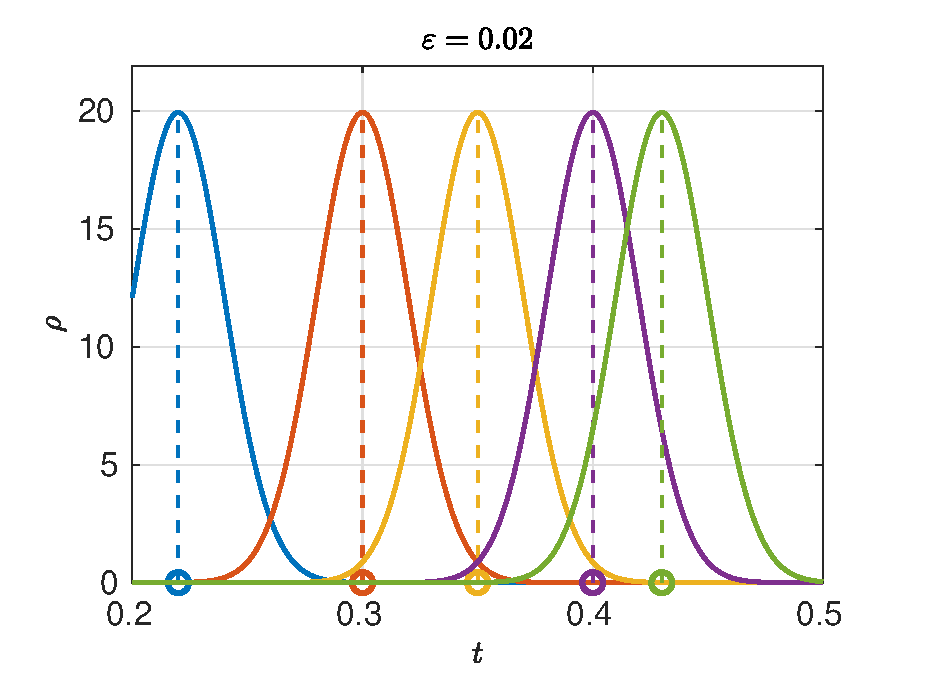
\includegraphics[width=0.7\textwidth]{./pics/peaks_med}
\end{center}
\caption{Разным цветам отвечают разные эксперименты. Для каждого эксперимента: проколотый круг на оси Х -- наше предсказание ответа, купол -- распределение плотности вероятности того, что истинное значение ответа примет значение $t$, в зависиомсти от $t$.} \label{img:peaks_med}
\end{figure}

На Рис. \ref{img:peaks_med} видно, что для всех точек кроме синей почти вся кривая (вероятность = площать под кривой) находится в исследуемом интервале. Это значит, что при $\varepsilon = 0.02$ для всех точек кроме синей вероятность того, что интинное значение параметра попадет в интервал, равна почти 100\%. Синяя же точка находится на расстоянии $\sim 1 \sigma$ (в данном случае 0.02), что значит, что вероятность того, что истинное значение параметра в синем эксперименте попадет в интервал $[0.2; 0.5]$ будет $\approx 16 \%$. Попадания истинных значений в интервал -- события независимые, поэтому вероятность реализации картины в целом будет произведением вероятностей попадания каждого значения в интервал по отдельности. В нашем случае все вероятности кроме синей $\approx 1$, поэтому общая вероятность $\approx$ синяя вероятность $\approx$ 0.84\%. Это значит, что если бы погрешность нашей программы была 0.02, то вероятность случатся тому что случилось на рассматриваемых 5 экспериментах в совокупности была бы = 84 \%. Поняв это, можно решить обратную задачу: сказать, что мы верим эксперименту на скажем 95\%, и найти такое $\varepsilon$, при котором вероятность его реализации как раз будет = 95\%. Понятно, что задача решаема -- если в предыдущем примере мы возьмем $\varepsilon = 0.008$, то распределение вероятностей для истинных значений будет 

\begin{figure}[h!]
\begin{center}
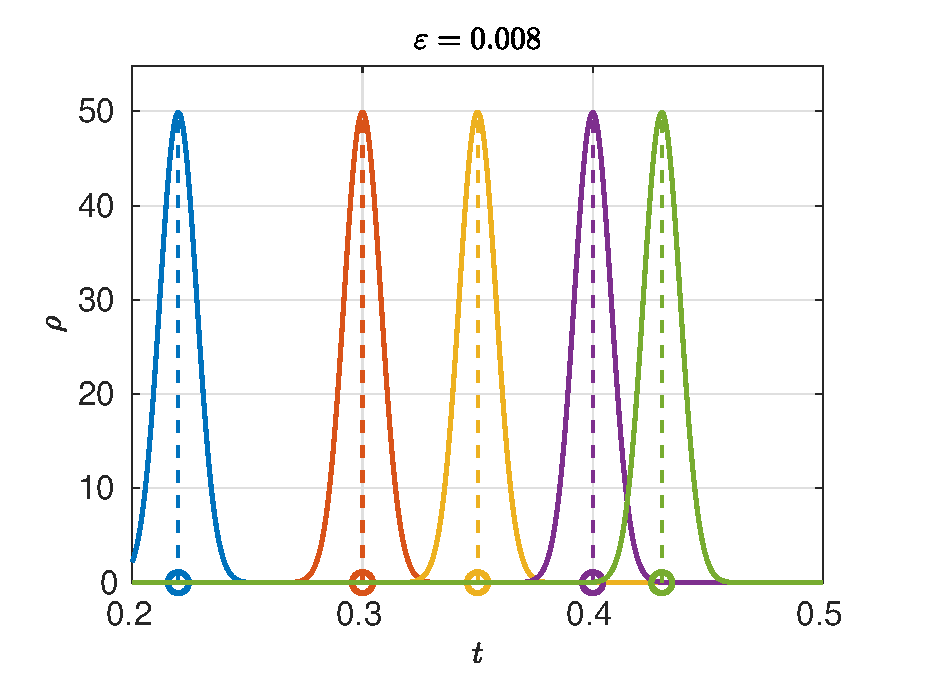
\includegraphics[width=0.7\textwidth]{./pics/peaks_sharp_med}
\end{center}
\caption{Обозначения аналогичны Рис. \ref{img:peaks_med}. Вероятность реализации эксперимента >99\%.} \label{img:peaks_sharp_med}
\end{figure}

\newpage

Если же все наши экспериментальные точки лежат ближе к центру исследуемой области, то оценка на погрешность выходит грубой. Это понятно из следующего примера. Сдвинем точку 0.22 из предыдущего примера в точку 0.28. График для $\varepsilon = 0.04$ будет выглядить как

\begin{figure}[h!]
\begin{center}
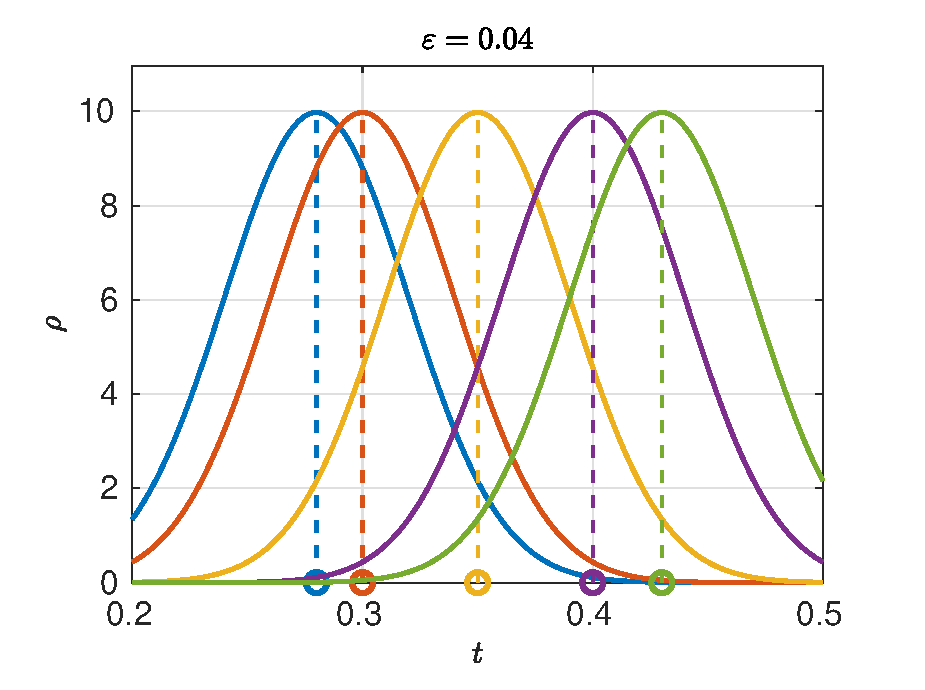
\includegraphics[width=0.7\textwidth]{./pics/peaks_smooth}
\end{center}
\caption{Обозначения аналогичны Рис. \ref{img:peaks_med}. Вероятность реализации эксперимента 92.5\%.} \label{img:peaks_smooth}
\end{figure}

Т.е. при налиции точки 0.22, близкой к левой границе иследуемого интервала 0.2, вероятность реализации эксперимента уже при $\varepsilon = 0.02$ была 84\%, что говорило о том, что в реальности скорее всего погрешность была меньше. Здесь же даже при $\varepsilon = 0.04$ вероятность все еще >90\%. Это на самом деле логично, т.к. если все наши точки у центра интервала, то единственный известный нам факт (на котором и строится вся оценка опгрешности) о том, что все истинные значения попали в интервал, поволяет отбросить только самые большие значения погрешностей.

При желании 

Теперь приведем аналитическое выражение описанной идеи:

\newpage

\subsection{Расчет}

Вероятность попадание $i$-ой истинной точки в интервал

\begin{equation}
p_i(\varepsilon) = \int\limits_a^b g \left(x, x_i, \varepsilon \right) dx = \int\limits_{(a-x_i)/\varepsilon}^{(b-x_i)/\varepsilon} g(x, 0, 1) dx.
\end{equation}

Введем функцию ошибок

\begin{equation}
\textsf{erf}(x) = \int\limits_{- \infty}^x g(t, 0, 1) dt.
\end{equation}

Попадание каждого истинного значения в интервал - независимое событие, поэтому вероятность реализации нашей совокупности экспериментов

\begin{equation}
p(\varepsilon) = \prod_{i = 1}^N p_i(\varepsilon) = \prod_{i = 1}^N \left[ \textsf{erf} \left( \dfrac{b - x_i}{\varepsilon} \right) - \textsf{erf} \left( \dfrac{a - x_i}{\varepsilon} \right) \right]
\end{equation}

Для нахождения желаемого $\varepsilon_0$ решаем уравнение $p(\varepsilon_0) = p_0$. 

Очевидно, что

\begin{equation} 
\left.
\begin{aligned} 
\forall \varepsilon > 0 \hspace{10pt} p'(\varepsilon) < 0 & \\
\text{ran} [p(\varepsilon)] = (0;1) & \\
\end{aligned}
\right\} \Rightarrow \hspace{10pt} \forall p_0 \in (0;1) \hspace{6pt} \exists ! \hspace{3pt} \varepsilon > 0 : p(\varepsilon) = p_0,
\end{equation}

поэтому $\forall p_0 \in (0;1)$ уравнение хорошо решается численно.

\subsection{Пример}

Для примера можно взять случайный набор из 10 точек в интервале $[0.25 \cdot 1.05; \hspace{5pt} 0.5 \cdot 0.95]$ и считать, что их истинные значения принаждежат $[0.25; 0.5]$.

\newpage

\begin{figure}[h!]
\begin{center}
\includegraphics[width=1\textwidth]{./pics/rand_line}
\end{center}
\caption{Расположение 10 пробных точек в интервале $[0.25; 0.5]$.} \label{img:rand_line}
\end{figure}

\begin{figure}[h!]
\begin{center}
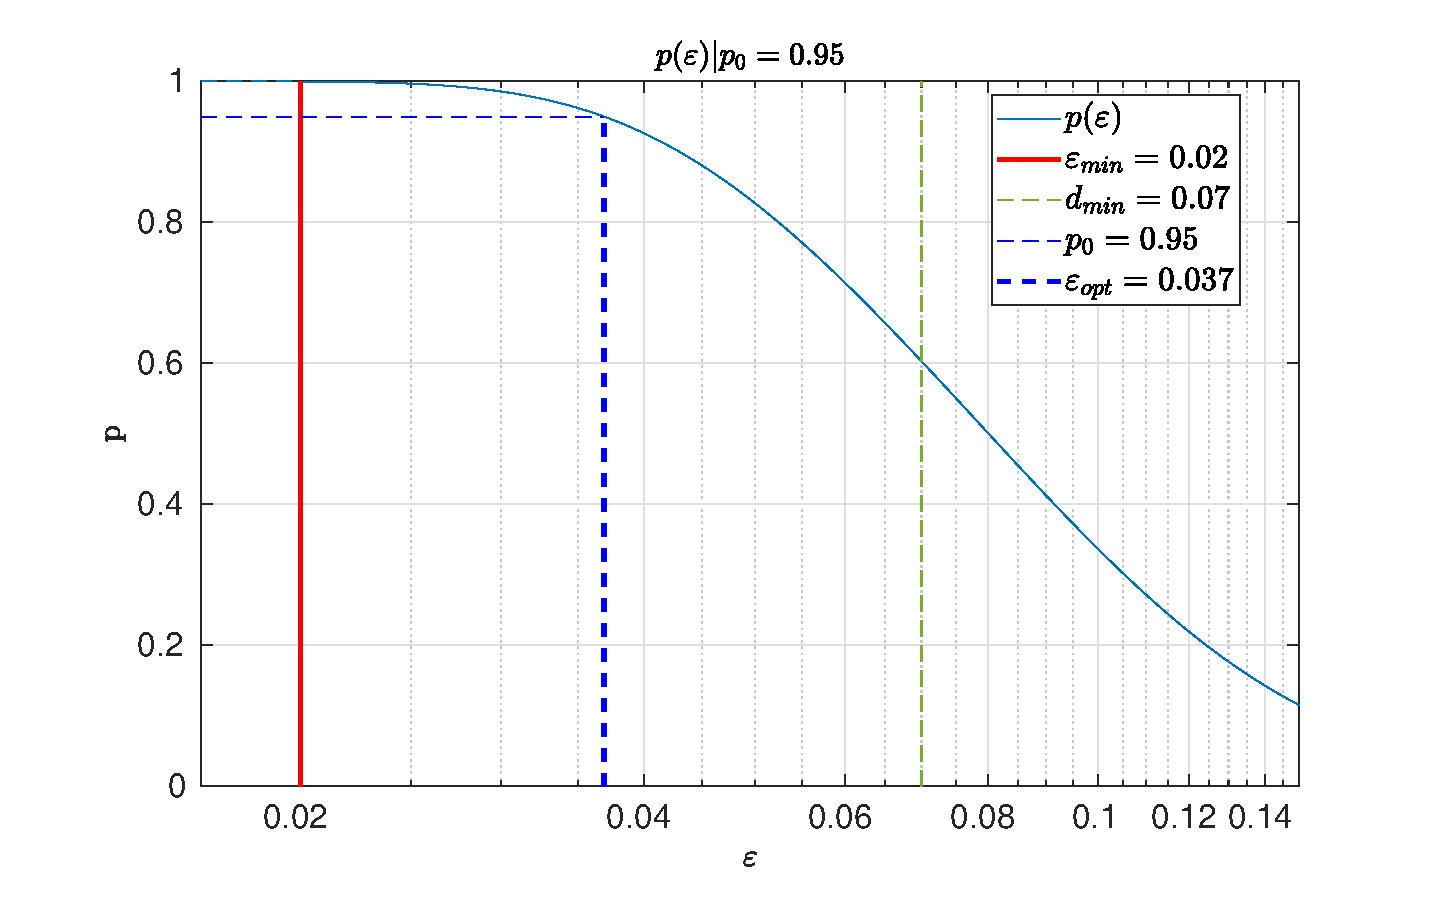
\includegraphics[width=1\textwidth]{./pics/vis}
\end{center}
\caption{Зависимость $p(\varepsilon)$. Красная линия -- принятая минимально возможная погрешность $\varepsilon_{min} = 0.02$, Синяя вертикаль -- найденная оценка, синяя горизонталь --наш выбор $p_0 = (1 - \mathcal{P}_{gauss}(1\sigma))/2$, зеленый пунктир - минимальное расстояние точек до границы. Видно, что наличие множества точке позволяет улучшить оценку с очевидного значения минимального расстояния до границы -- линяя линия левее зеленой.} \label{img:vis}
\end{figure}

\section{Результат применения}

Можно исследовать, как оценка погрешности зависит от количества имеющихся экспериментальных данных в <<усредненном>> случае, когда ответы нашей программы расположены в интервале на равных промежутках.

\begin{figure}[h!]
\begin{center}
\includegraphics[width=1\textwidth]{./pics/uni_line}
\end{center}
\caption{Равномерное расположение 10 пробных точек в интервале $[0.25; 0.5]$.} \label{img:uni_line}
\end{figure}

\begin{figure}[h!]
\begin{center}
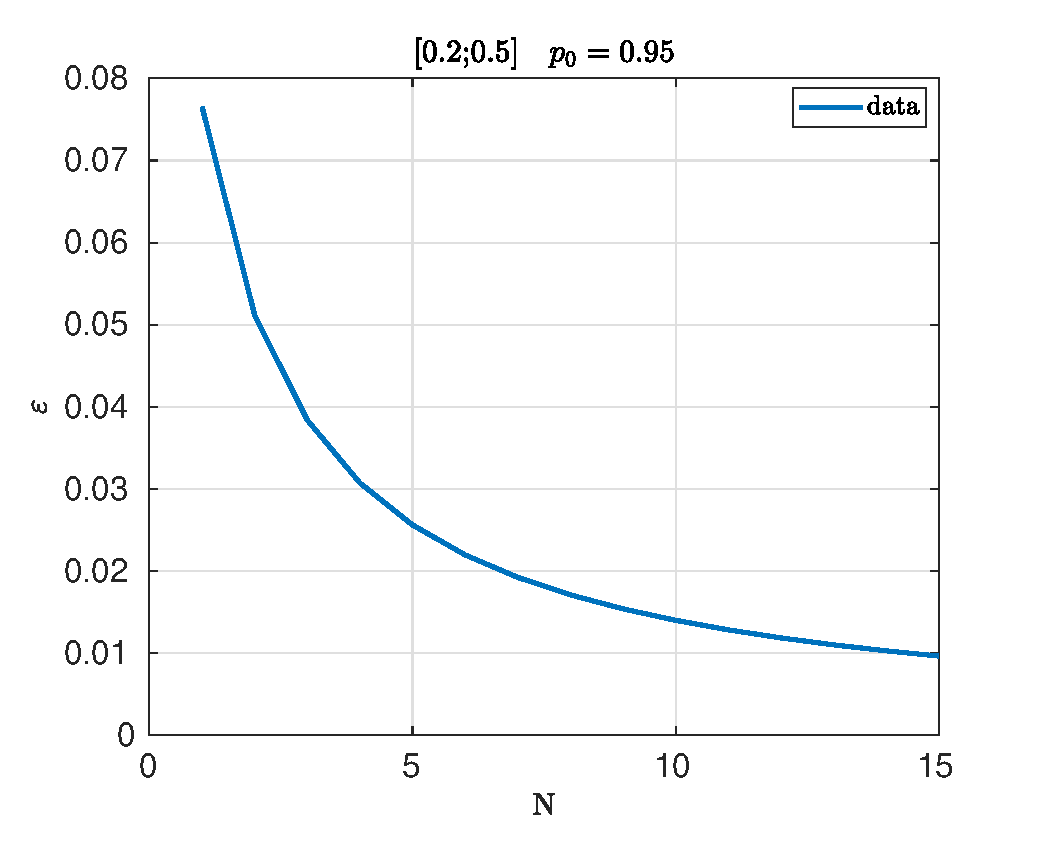
\includegraphics[width=1\textwidth]{./pics/linear}
\end{center}
\caption{$\varepsilon(N)$} \label{img:linear}
\end{figure}

На глаз зависимость на рис.(\ref{img:linear}) близка к $1/N$, что ожидаемо, т.к. погрешность в основном определяется минимальным расстояние до границы, которое при выбранной расстановке точек убывает как $1/N$. 

Можно проверить отклонения от закона $1/N$ -- рис.(\ref{img:log}).

\begin{figure}[h!]
\begin{center}
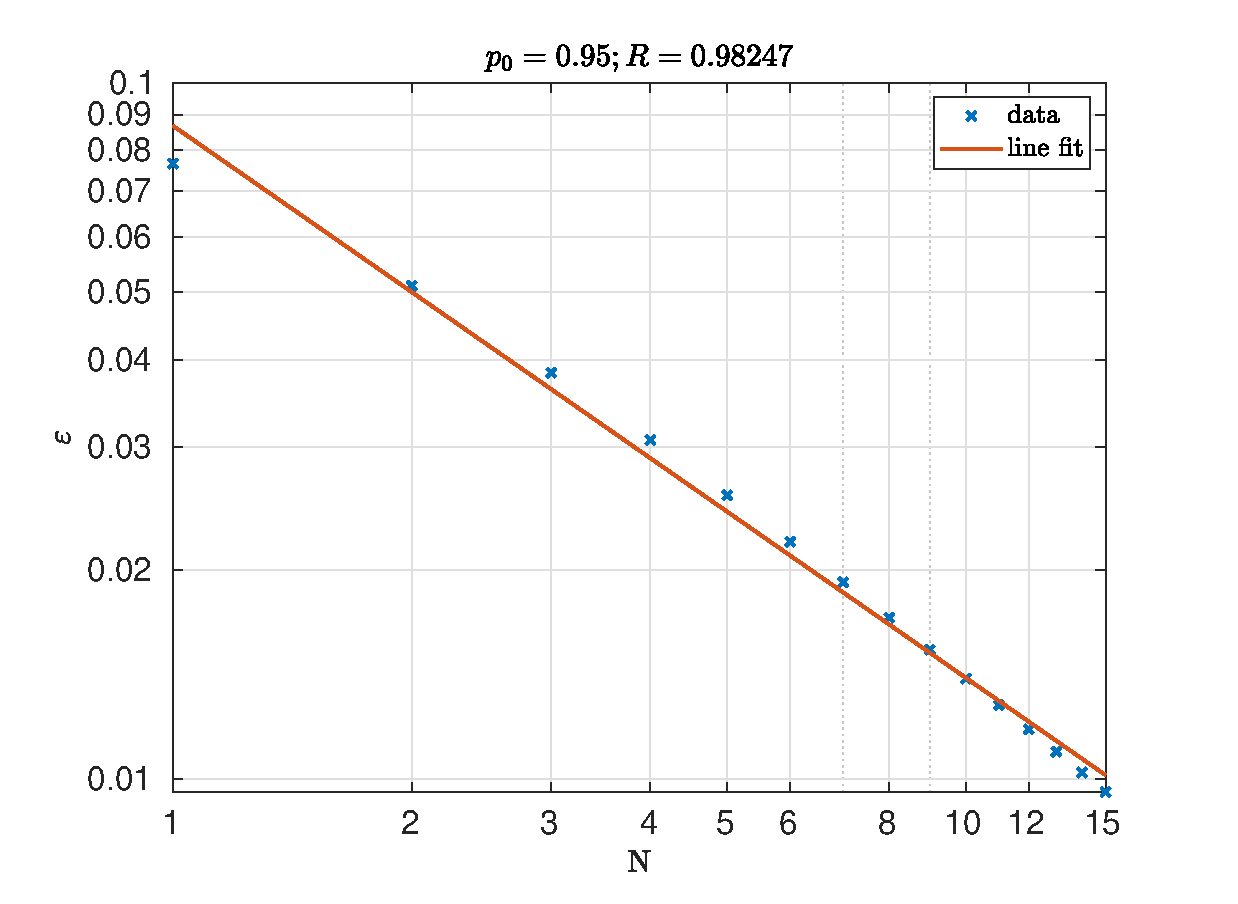
\includegraphics[width=1\textwidth]{./pics/log}
\end{center}
\caption{$\varepsilon(N)$, логарифмический масштаб, попытка линеаризации} \label{img:log}
\end{figure}

Видно, что наклон с правда близок к $-1$, но небольшие отклонения от линейности есть.

\end{document} % конец документа